
\chapter{Estado del Arte}


\par Actualmente, el desarrollo y uso de la inteligencia artificial está en boca de todos, pero ¿qué es esta famosa 
inteligencia artificial y por qué ha adquirido tanta relevancia recientemente? A pesar de que ha sido desafiante
definir este concepto durante mucho tiempo, podemos decir que la inteligencia artificial, también conocida 
como inteligencia de máquina (Machine Learning en inglés), es el uso de la inteligencia demostrada por la 
tecnología y maquinas \cite{mt1}. En general, la inteligencia artificial, abreviada como AI (del inglés Artificial Intelligence) 
o IA (de la palabra en español), engloba técnicas como el aprendizaje automático, el aprendizaje profundo y
otros aspectos de la inteligencia artificial \cite{mt1}. Estos temas no son nuevos y han sido objeto de estudio durante 
muchos años. Por ejemplo, en el caso del aprendizaje profundo (Deep Learning en inglés), este se basa en el 
perceptrón, que fue descubierto en 1958 \cite{perceptron}, por lo que no es un descubrimiento reciente. No fue hasta nuestros tiempos, cuando el poder de cómputo y las interfaces 
han sido democratizadas para el común de los usuarios, que hemos podido experimentar y entender realmente lo que la 
inteligencia artificial puede realizar por nosotros.\\


\begin{figure}[ht!]
    \centering
    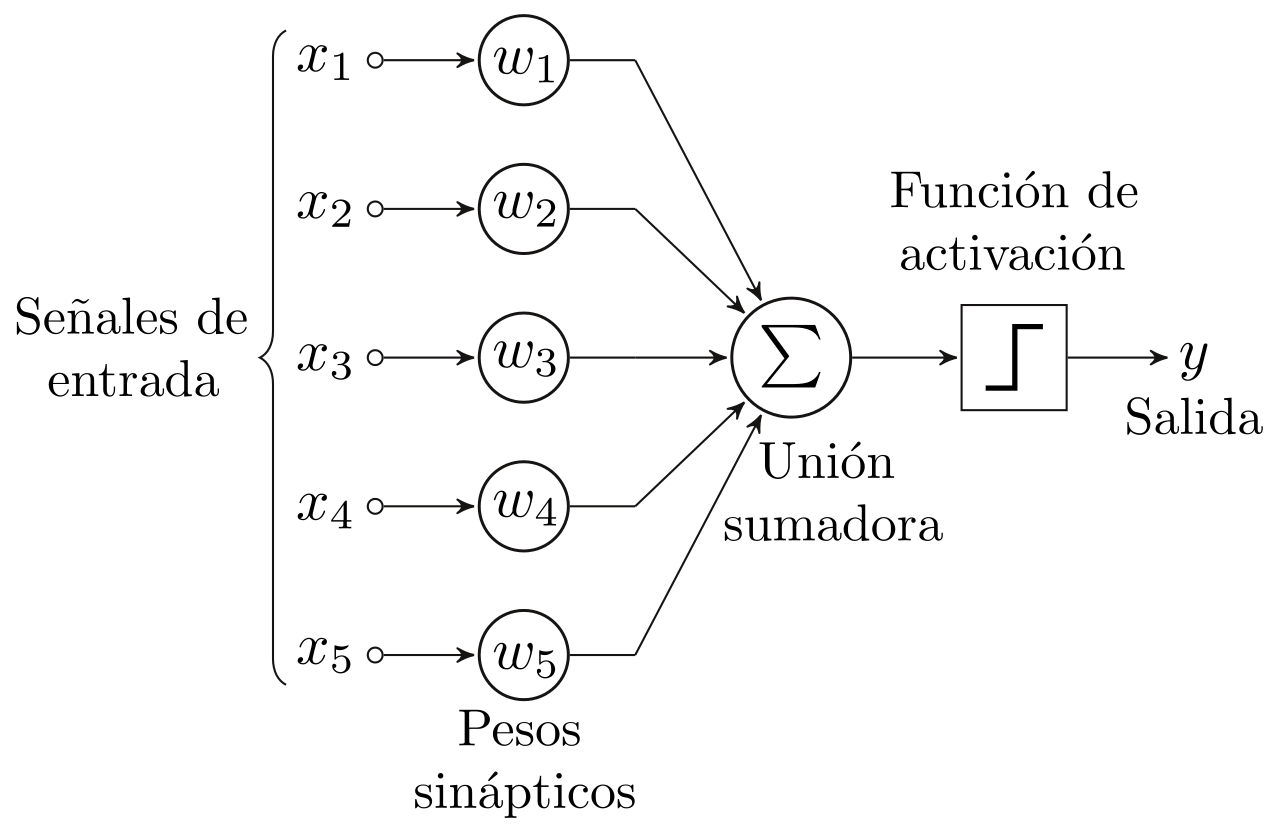
\includegraphics[width=.75\textwidth]{figures/ea1.png}
    \caption[Estructura del perceptrón]{Diagrama de un perceptrón,\\
    {\scriptsize (Fuente: Wikipedia)}}
    \label{fig:ea1}
\end{figure}

\newpage

\par Luego de entender lo que es la inteligencia artificial queda la pregunta ¿Qué es lo diferente actualmente que no era capaz de ofrecer en el pasado? 
El 30 de noviembre de 2022 fue abierto al público la aplicación ChatGPT por la empresa especialista en inteligencia artificial OpenAI \cite{mt3}, deslumbrando a todos 
con la capacidad de responder las preguntas que los usuarios les entregaban, elevando aún más el interés por esta empresa y por este tipo de tecnología.
La base de esta herramienta nace de una rama específica de la inteligencia artificial llamada procesamiento del lenguaje 
natural, abreviado NLP, en si siglas en inglés Natural Language Processing, siendo este un subcampo de la Inteligencia Artificial y lingüístico, dedicado a hacer que las 
computadoras comprendan declaraciones o palabras escritas en lenguajes humanos \cite{nlpeda}, llevando así el estudio de no solo texto sino de la lingüística y la sintaxis que los textos contienen.


\par El verdadero impacto que provocó ChatGPT en el mundo, fue el conocimiento popular de lo que hoy llamamos inteligencia 
artificial generativa, que puede ser definida como una técnica de inteligencia artificial que genera artefactos sintéticos analizando 
ejemplos de entrenamiento; aprendiendo sus patrones y distribución; y luego creando facsímiles realistas. La inteligencia 
artificial generativa (GAI) utiliza la modelización generativa y los avances en el aprendizaje profundo (DL) para producir 
contenido diverso a gran escala utilizando medios existentes como texto, gráficos, audio y video \cite{mt2}. Por lo que, el público en
general pudo entender que existían herramientas que podían crear diversos contenidos y con ello el boom de estas 
tecnologías entre la población fue cada vez más grande. \\


\begin{figure}[ht!]
    \centering
    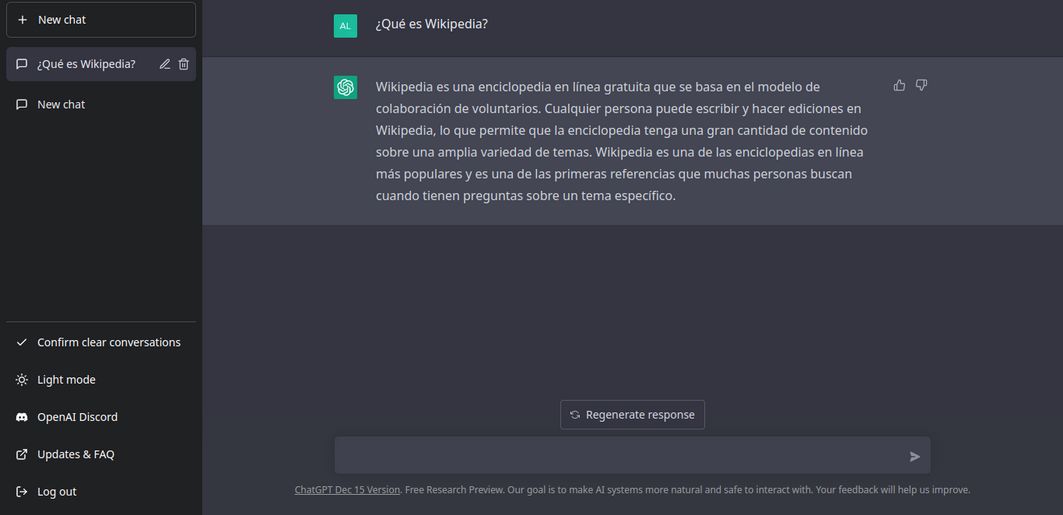
\includegraphics[width=.8\textwidth]{figures/ea2.png}
    \caption[Screenshot de la pagina de ChatGPT]{Screenshot de la pagina de ChatGPT \\
    {\scriptsize (Fuente: ChatGPT)}}

    \label{fig:ea2}
\end{figure}

\par Cuando hablamos de inteligencia artificial y sus aplicaciones, usualmente nos referimos a la generación de diferentes modelos. Sin embargo,
en el contexto de la inteligencia artificial generativa, como las herramientas que producen texto o asisten en problemas de 
Procesamiento de Lenguaje Natural (NLP, por sus siglas en inglés), también estamos hablando de un modelo de inteligencia 
artificial. La diferencia radica en que estos son considerablemente más grandes en términos del volumen de datos que manejan. 
Dado que están enfocados en temas de lenguaje, comúnmente los denominamos modelos grandes de lenguaje o LLM, por sus siglas 
en inglés de ``Large Language Models'', siendo estos formalmente definidos como herramientas de inteligencia artificial (AI) 
basadas en redes neuronales recurrentes multicapa que son entrenadas con vastas cantidades de datos para generar texto 
similar al humano \cite{mt6}.

\begin{figure}[ht!]
    \centering
    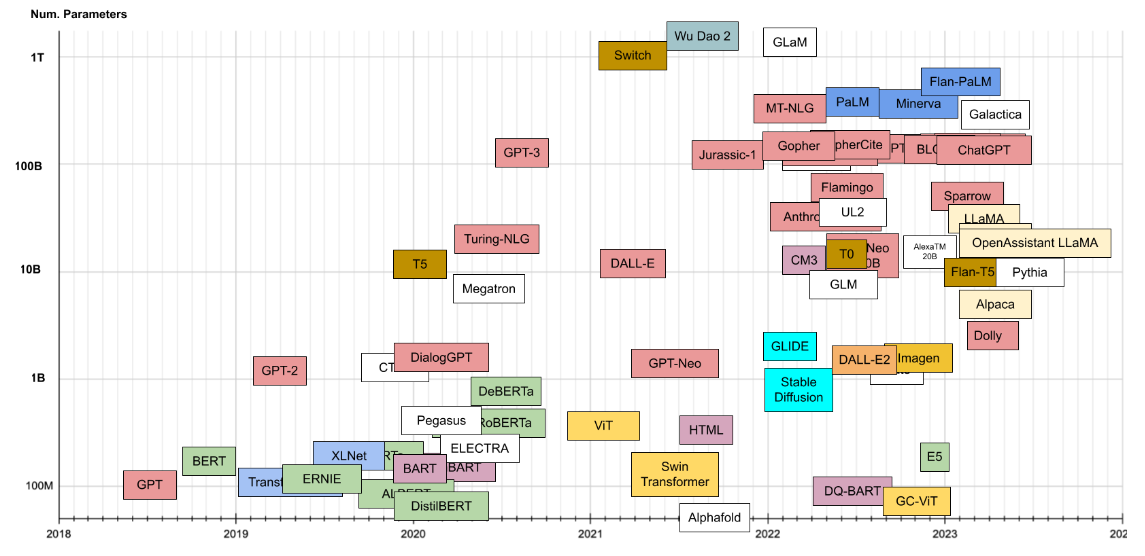
\includegraphics[width=0.7\textwidth]{figures/ea4.png}
    \caption[Línea de tiempo del Transformer]{Línea de tiempo del Transformer. En el eje vertical, número de parámetros.
    Los colores describen la familia Transformer,\\
    {\scriptsize (Fuente: Transformer models: an introduction and catalog \cite{eb4})}}

    \label{fig:ea3}
\end{figure}

\newpage

\par ChatGPT funciona mediante una arquitectura base llamada Transformer \cite{aiayn}, arquitectura creada por Google, que ha generado 
la gran revolución en la inteligencia artificial como la conocemos hasta la fecha, debido a que no necesariamente se centra en NLP, 
sino en inteligencia artificial generativa en general. Si somos aún más específicos, GPT viene de Transformer generativo 
pre entrenado, ``Generative Pre-trained Transformer'' en inglés, siendo esta una arquitectura con habilidad de comprender el 
lenguaje de mejor manera usando la arquitectura de los Transformers \cite{mt4}. Aunque no fue hasta que este modelo creció hasta una cierta cantidad de parámetros que 
pudo demostrar sus capacidades en la gran amalgama de tareas que existen en el procesamiento de lenguaje natural, incluyendo la generación de texto como tal \cite{mt5}.


\begin{figure}[ht!]
    \centering
    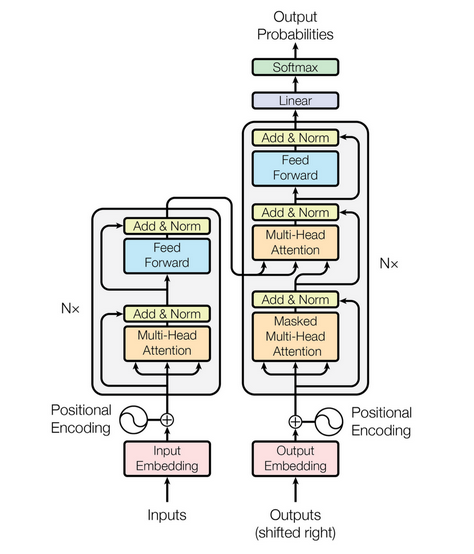
\includegraphics[width=.5\textwidth]{figures/ea3.png}
    \caption[Diagrama de la arquitectura un Transformer]{Diagrama de la arquitectura un Transformer,\\
    {\scriptsize (Fuente: Attention Is All You Need \cite{aiayn})}}
    \label{fig:ea4}
\end{figure}

\newpage

Complementado lo anterior, es importante entender el funcionamiento de estos modelos ¿Cómo es posible que logren entender lo que escribo? Los modelos 
GTP funcionan en base a redes neuronales las cuales no entienden ni de letra y palabras, por lo que este texto tiene que pasar por
una función de Embedding. Embedding es el proceso en el que representamos un texto, párrafo o documento de manera numérica, siendo
esta representación en vector de múltiples dimensiones \cite{eb1}, estos vectores se pueden ``graficar'' en un espacio multi dimensional y con 
ello es posible ver la cercanía de cada uno de estos vectores entre ellos, por lo que este vector sirve como punto de entrada para
el funcionamiento de los modelos GTP \cite{eb2}. Además, se suelen usar para tareas como búsqueda, agrupación, recomendaciones, 
búsqueda de anomalías, etc \cite{eb3}.

\begin{figure}[ht!]
    \centering
    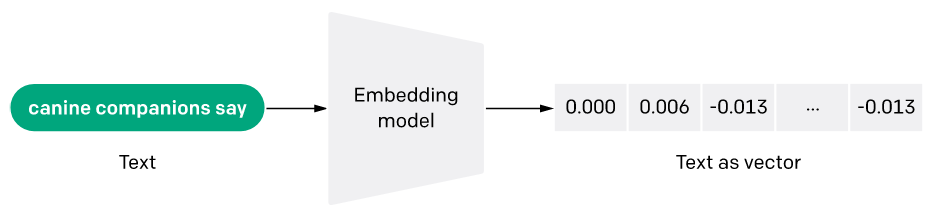
\includegraphics[width=.8\textwidth]{figures/huemul4.png}
    \caption[Diagrama del funcionamiento de un Embedding]{Diagrama del funcionamiento de un Embedding,\\
    {\scriptsize (Fuente: OpenAI\cite{openai1})}}
    \label{fig:ea5}
\end{figure}

Finalmente, todos estos conceptos nos ayudarán a entender el trasfondo de todas estas tecnologías y como estas interactúan 
con un Chatbot ¿Pero qué es un Chatbot? Para ello, primero será necesario entender que denominamos prompt, a pesar de que 
no existe una definición como tal, podríamos decir que son instrucciones textuales y ejemplo de interacciones deseadas 
que se antepone a las entradas de los modelos grandes de lenguaje, estos pueden sesgar los modelos y generar salidas 
deseadas, mejorando así la calidad de las salidas que generan estos modelos \cite{prompt}, esto es importante porque dependiendo 
que y como es la pregunta, o input, que se da a un modelo grande de lenguaje este puede tener una mejor o peor respuesta. 
Estos prompt son importantes porque son lo que recibe el chatbot, que esta potenciado por los LLM, por lo que podemos 
definir un chatbot como un programa informático diseñado para simular conversaciones con usuarios humanos \cite{chatbot_def}, especialmente 
a través de Internet, que será el proyecto que acompaña a esta tesis. 

